\begin{figure}[htbp]
    \centering
    \begin{subfigure}[b]{0.95\textwidth}
    \centering
    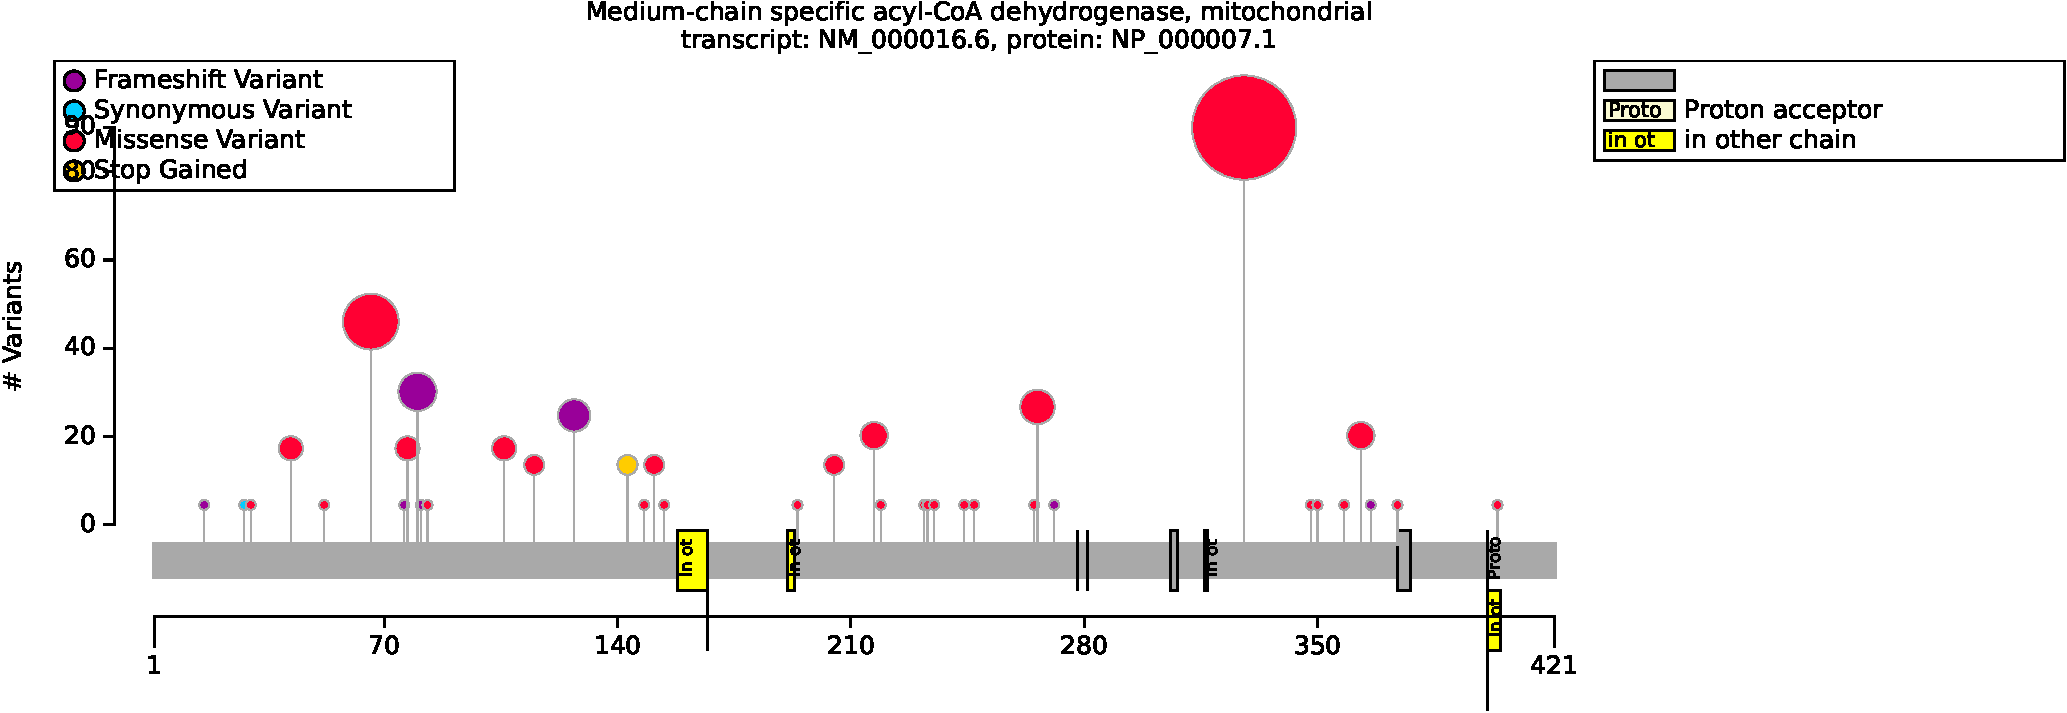
\includegraphics[width=\textwidth]{ img/ACADM_protein_diagram.pdf} 
    \captionsetup{justification=raggedright,singlelinecheck=false}
    \caption{Distribution of variants in ACADM}
    \end{subfigure}
    
    \vspace{2em}

    \begin{subfigure}[b]{0.95\textwidth}
    \centering
    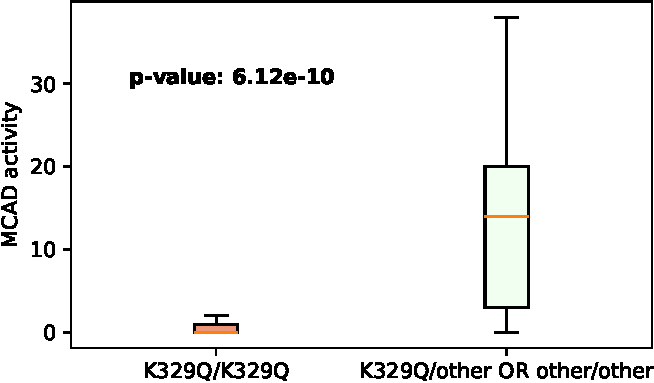
\includegraphics[width=0.3\textwidth]{ img/acadm_k329q.pdf} 
    \captionsetup{justification=raggedright,singlelinecheck=false}
    \caption{Lys329Glu: t test for MCAD Activity (\% normal; LOINC:74892-1): p=$6.12\times 10^{-10}$.}
    \end{subfigure}
    
    \vspace{2em}
    
    \begin{subfigure}[b]{0.95\textwidth}
    \captionsetup{justification=raggedright,singlelinecheck=false}
    \resizebox{\textwidth}{!}{
    \begin{tabular}{llllrr}
    \toprule
    Description & Variable & Genotype (A) & Genotype (B) & p-value & xrefs\\
    \midrule
    Value of MCAD Activity\% [LOINC:74892-1] & LOINC:74892-1 & K329Q/K329Q & K329Q/other OR other/other & $6.12\times 10^{-10}$ & \cite{PMID_33580884}\\
    \bottomrule
    \end{tabular}
    }
    \caption{t-test to compare K329Q/K329Q and K329Q/other OR other/other with respect to LOINC:74892-1. Mean MCAD activity for K329/K329: 0.52\%, and for K329/other or other/other: 13.23\% }
    \end{subfigure}
    
    \vspace{2em}
    
    \begin{subfigure}[b]{0.95\textwidth}
    \captionsetup{justification=raggedright,singlelinecheck=false}
    \resizebox{\textwidth}{!}{
    \begin{tabular}{llllrr}
    \toprule
    Description & Variable & Genotype (A) & Genotype (B) & p-value & xrefs\\
    \midrule
    Value of MCAD Activity\% [LOINC:74892-1] & LOINC:74892-1 & Y67H/Y67H OR Y67H/other & other/other & $2.01\times 10^{-5}$ & \cite{PMID_33580884}\\
    \bottomrule
    \end{tabular}
    }
    \caption{t-test to compare Y67H/Y67H OR Y67H/other and other/other with respect to LOINC:74892-1. Mean MCAD activity for Y67H/Y67H: 18.60\%, and for Y67H/other or other/other: 7.68\% }
    \end{subfigure}
    
    \vspace{2em}
    
    \caption{The cohort comprised 115 individuals (0 females, 0 males, 115 with unknown sex). The cohort had data about  medium chain Acyl-CoA dehydrogenase (MCAD), expressed as percentage of normal.
    The variant c.985G$>$A (p.Lys329Glu) is known to be severe, and the variant c.199T$>$C (p.Tyr67His) is known to be mild \cite{PMID_33580884}.
    Disease diagnosis: Acyl-CoA dehydrogenase, medium chain, deficiency of (OMIM:201450). No statistically significant results identified. A total of 188 unique variant alleles were found in \textit{ACADM} (transcript: \texttt{NM\_000016.6}, protein id: \texttt{NP\_000007.1}).}
    \end{figure}
    